\documentclass[12pt]{article}
 
\usepackage[margin=1in]{geometry} 
\usepackage{amsmath,amsfonts,amsthm,amssymb}
\usepackage{mathtools}
\usepackage{pifont}
\usepackage{graphics}
\usepackage{graphicx}
\usepackage{array}
\usepackage{listings}
\usepackage{matlab-prettifier}
\usepackage[hidelinks]{hyperref}
\usepackage{caption}
\usepackage{enumitem}

\lstdefinestyle{tex-style} {
	language=Matlab,                           % Code langugage
	basicstyle=\ttfamily,                   % Code font, Examples: \footnotesize, \ttfamily
	%keywordstyle=\color{OliveGreen},        % Keywords font ('*' = uppercase)
	commentstyle=\color{gray},              % Comments font
	numbers=none,                           % Line nums position
	numberstyle=\tiny,                      % Line-numbers fonts
	stepnumber=1,                           % Step between two line-numbers
	numbersep=5pt,                          % How far are line-numbers from code
	%backgroundcolor=\color{gray}, % Choose background color
	frame=single,                             % A frame around the code
	tabsize=2,                              % Default tab size
	captionpos=b,                           % Caption-position = bottom
	breaklines=true,                        % Automatic line breaking?
	breakatwhitespace=false,                % Automatic breaks only at whitespace?
	showspaces=false,                       % Dont make spaces visible
	showtabs=false,                         % Dont make tabls visible
	columns=flexible,                       % Column format
	morekeywords={__global__, __device__}  % CUDA specific keywords
}
\lstset{style=tex-style}
 
\newcommand{\N}{\mathbb{N}}
\newcommand{\Z}{\mathbb{Z}}
 
\newenvironment{theorem}[2][Theorem]{\begin{trivlist}
\item[\hskip \labelsep {\bfseries #1}\hskip \labelsep {\bfseries #2.}]}{\end{trivlist}}
\newenvironment{lemma}[2][Lemma]{\begin{trivlist}
\item[\hskip \labelsep {\bfseries #1}\hskip \labelsep {\bfseries #2.}]}{\end{trivlist}}
\newenvironment{exercise}[2][Exercise]{\begin{trivlist}
\item[\hskip \labelsep {\bfseries #1}\hskip \labelsep {\bfseries #2.}]}{\end{trivlist}}
\newenvironment{problem}[2][Problem]{\begin{trivlist}
\item[\hskip \labelsep {\bfseries #1}\hskip \labelsep {\bfseries #2.}]}{\end{trivlist}}
\newenvironment{question}[2][Question]{\begin{trivlist}
\item[\hskip \labelsep {\bfseries #1}\hskip \labelsep {\bfseries #2.}]}{\end{trivlist}}
\newenvironment{corollary}[2][Corollary]{\begin{trivlist}
\item[\hskip \labelsep {\bfseries #1}\hskip \labelsep {\bfseries #2.}]}{\end{trivlist}}

\newenvironment{solution}{\begin{proof}[Solution]}{\end{proof}}

%%%%%%% Table Packages %%%%%%%%%%%%%%%%%%%%%%%
\usepackage{booktabs}
\usepackage{multirow}
\usepackage{array}
\usepackage[T1]{fontenc}
\usepackage[utf8]{inputenc} 
\usepackage{tabularx,ragged2e,booktabs}
\newcolumntype{C}[1]{>{\Centering}m{#1}}
\renewcommand\tabularxcolumn[1]{C{#1}}
\newcommand{\ra}[1]{\renewcommand{\arraystretch}{#1}}
\usepackage{makecell}
\usepackage{tikz}
\usetikzlibrary{tikzmark,calc}
\usepackage{siunitx}
\usepackage[hidelinks]{hyperref}
\usepackage{amsmath}

 
\begin{document}
 
% --------------------------------------------------------------
%                         Start here
% --------------------------------------------------------------
 
\title{Homework 4}
\author{MEGN544/ROBO554 Robot Mechanics: Kinematics, Dynamics, and Control  
\\ 
Dr. George Kontoudis\\
Department of Mechanical Engineering\\
Colorado School of Mines}
\date{Fall 2026}
 
\maketitle
\begin{problem}{1}%theorem, exercise, problem, or question 
Derive from the inverse twist problem equations (p.~34 of notes) the
simplified forward and inverse equations for the twist parameterization in the
special case of parallel displacement $\boldsymbol{d}$ with the rotation axis $\widehat{\boldsymbol{k}}$.
 
\end{problem}

\begin{problem}{2}\label{p2}%theorem, exercise, problem, or question 
Sketch the zero-angle configuration from the following DH table.

\begin{table}[!h]
\centering
\begin{tabular}{c | c | c | c | c}
\hline 
 {Link} & $a$ & $d$ & $\alpha$ & $\theta$\\  \hline
 $1$ & $1$ & $1$ & $\pi/2$ & $\star$ \\ 
 $2$ & $0.5$ & $1$ & $-\pi/2$ & $\star$ \\ 
 $3$ & $0$ & $0$ & $0$ & $\star$ \\ 
 $4$ & $1$ & $0$ & $\pi/2$ & $\star$ \\ 
 $5$ & $0$ & $0$ & $-\pi/2$ & $\star$ \\ 
 $6$ & $0$ & $0$ & $\pi/2$ & $\star$ \\ \hline
\end{tabular}\label{tab:part_1_ii}
\end{table}
 
\end{problem}

\begin{problem}{3}\label{p3}%theorem, exercise, problem, or question 
Sketch the zero-angle configuration from the following DH table.

\begin{table}[!h]
\centering
\begin{tabular}{c | c | c | c | c}
\hline 
 {Link} & $a$ & $d$ & $\alpha$ & $\theta$\\  \hline
 $1$ & $1$ & $\star$ & $\pi/2$ & $0$ \\ 
 $2$ & $1$ & $\star$ & $\pi/2$ & $\pi/2$ \\ 
 $3$ & $1$ & $\star$ & $0$ & $0$ \\ \hline
\end{tabular}\label{tab:part_1_ii}
\end{table}
 
\end{problem}

\begin{problem}{4}%theorem, exercise, problem, or question 
For the manipulator of Problem~2:
\begin{enumerate}[label=(\alph*)]
    \item What is the homogeneous transformation $\prescript{0}{}{\boldsymbol{T}}_6 $ if all joint angles are 0?
    \item What is the homogeneous transformation $\prescript{0}{}{\boldsymbol{T}}_6 $ if all joint angles are $\pi/6$?
\end{enumerate}
 
\end{problem}

\begin{problem}{5}%theorem, exercise, problem, or question 
For the manipulator of Problem~3:
\begin{enumerate}[label=(\alph*)]
    \item What is $\prescript{0}{}{\boldsymbol{T}}_3$ when $d_1 = 1$ and all other joints are 0? 
    \item What is $\prescript{0}{}{\boldsymbol{T}}_3$ when $d_2 = 1$ and all other joints are 0? 
    \item What is $\prescript{0}{}{\boldsymbol{T}}_3$ when $d_3 = 1$ and all other joints are 0? 
\end{enumerate}
 
\end{problem}

\begin{problem}{6}%theorem, exercise, problem, or question 
Derive the DH parameters for the RRPR manipulator shown in Fig.~\ref{fig:p6}.
\begin{figure}[!h]
	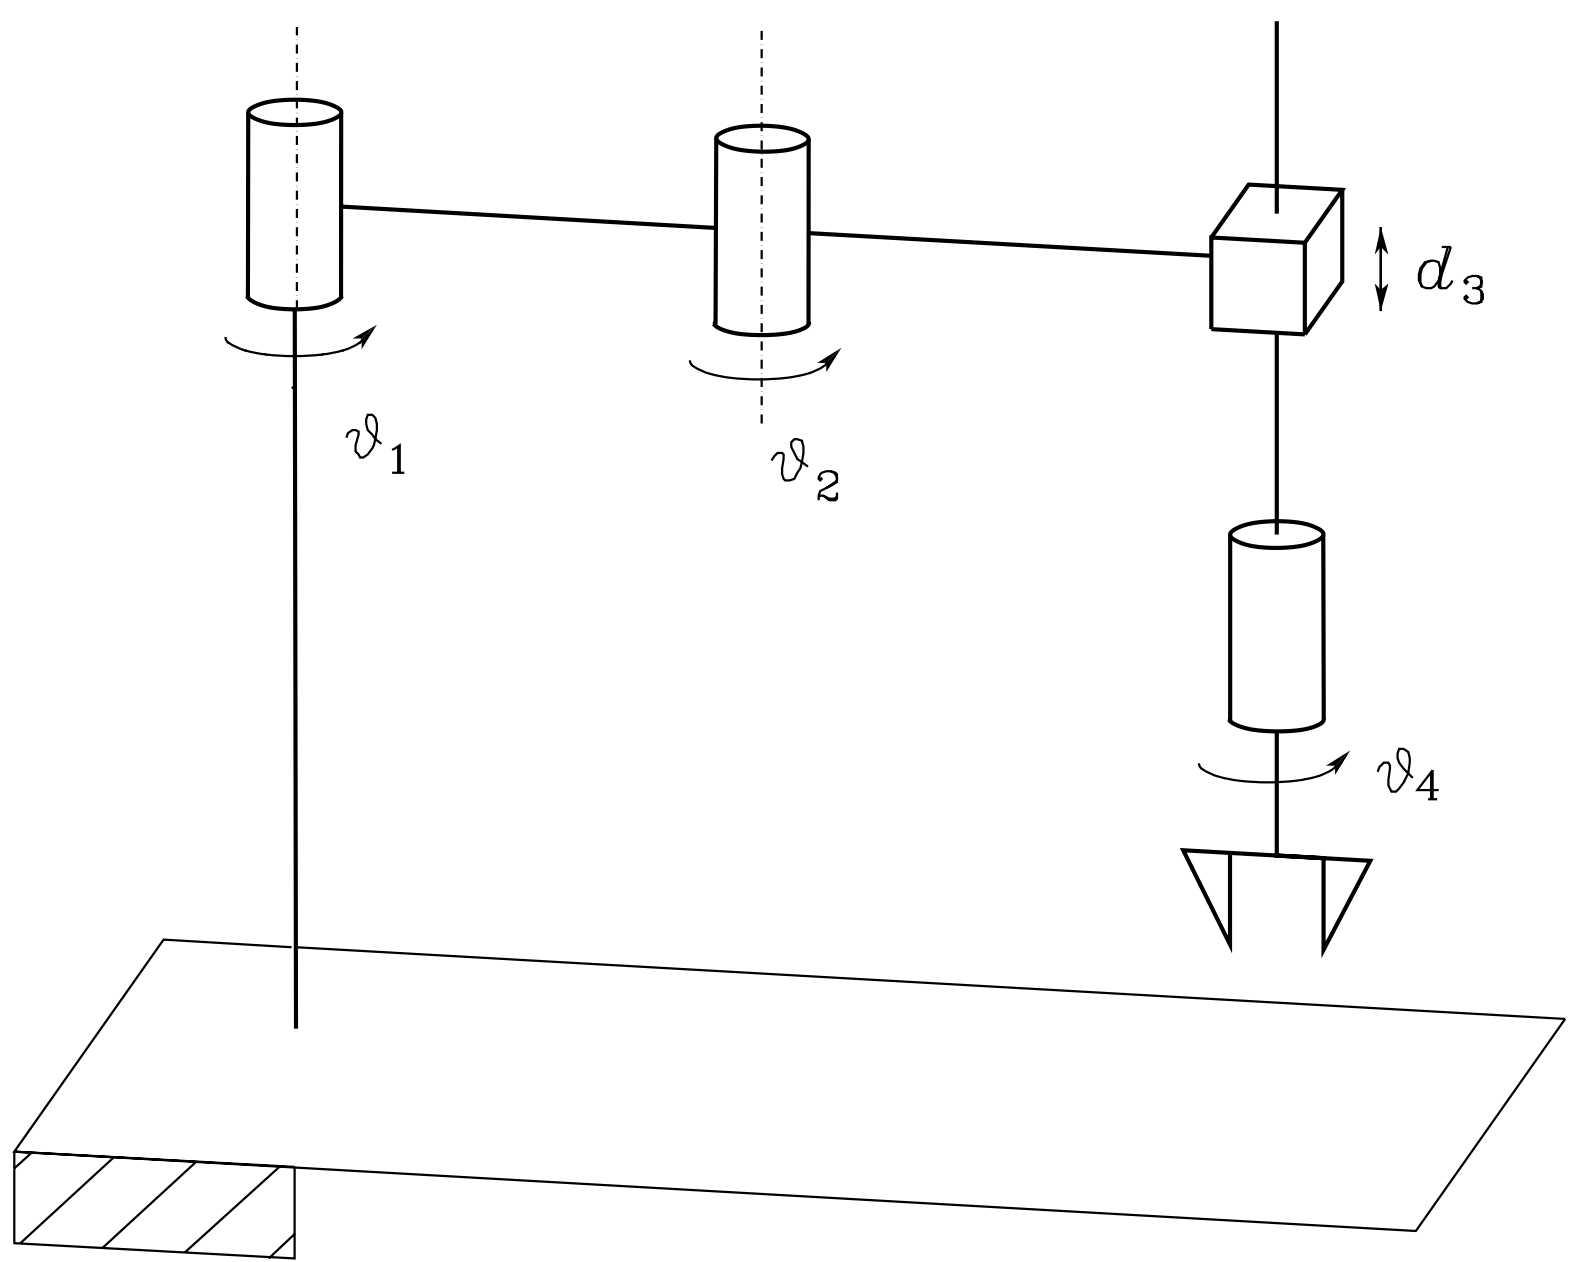
\includegraphics[width=.4\columnwidth]{figures/SCARA_manipulator_siciliano_fig_2.36.png}
	\centering
	\caption{RRPR manipulator.}
	\label{fig:p6}
\end{figure}
 
\end{problem}


\end{document}